% Alles zur Hardware und unseren Modifikationen
% Zuständig: Mihael
\chapter{Hardware}
\label{sec:hardware}
\section{Elegoo Tumbller Kit}
\label{subsec:elegoo_tumbller}
Um den Hardwareaufbau so einfach wie möglich zu gestalten,
entschieden wir uns dafür,
fertig entwickelte Kits online zu bestellen und dann zu modifizieren.
%
Die Wahl des Kits fiel letztendlich auf den ``Tumbller'' von Elegoo (Siehe Abbildung \ref{fig:elegoo_tumbller}).
%
Der Tumbller ist ein zweirädriger Roboter, welcher auf einer Ache balanciert.
%
Zur Kontrolle des unmodifizierten Kits gibt es eine Smartphone-App,
welche die Roboter über Bluetooth fernsteuern kann.
%
Da wir die Roboter über WLAN steuern wollten, 
und die Tumbller-Kits standardmäßig nur eine Bluetooth-Erweiterung eingebaut haben,
haben wir die mitgelieferten Arduino Nano durch ESP32-Boards im Arduino Nano-Format ersetzt.
%
Der unmodifizierte Elegoo Tumbler besteht aus einem Arduino Nano der zur Steuerung des gesamten Roboters verwendet wird. Einem MPU6050 (Gyroskop- & Beschleunigungssensor), der zur Erkennung der Achsen und Bewegungen verwendet wird (balancieren). Des Weiteren hat er auch zwei Gleichstrommotoren mit Hall-Encodern zur Messung der Raddrehung, diese Motoren werden mit dem TB6612FNG Motortreiber gesteuert. Zudem verfügt der Elegoo Tumbler über ein HC-06 Bluetooth-Modul, das zur Kommunikation mit dem Smartphone verwendet wird. Mithilfe des SR04 Ultraschallsensor ist der Roboter in der Lage, Abstände zu messen, was es ihm ermöglicht, Hindernisse zu erkennen und zu umgehen.  Zudem besitzt der Tumbler Infrarot-Sensoren (IR204C-A und IRM-56384), die es ihm ermöglichen, Hindernisse und Linien zu erkennen oder zu verfolgen. Durch den AMS1117 3.3V Spannungswandler wird die Spannung von dem Li-Ion-Akku, der als Hauptstromversorgung dient, heruntergestuft, sodass sie auch für das Bluetooth-Modul und die Sensoren verwendbar ist. Des Weiteren ist der Elegoo Tumbler mit mehreren Modi ausgestattet. Diese kann man entweder über die App oder direkt am Roboter über einen Taster steuern, zur Visualisierung der Modi hat der Elegoo Tumbler mehrere LEDs eingebaut.
\section{Subkomponenten}
\label{subsec:subkomponenten}
%
\subsection{PCB}
%
\subsection{MPU6050 (Gyroskop- & Beschleunigungssensor)}
%
\subsection{TB6612FNG (Motortreiber)}
%
\subsection{AMS1117 (3.3V Spannungsregler)}
%
\subsection{HC-06 (Bluetooth Modul)}
%
\subsection{Arduino Nano (Microcontroller)}
%
\subsection{SR04 (Ultraschallsensor)}
%
\subsection{Infrarot-Sensoren (IR204C-A & IRM-56384)}
%
\subsection{Gleichstrommotoren (TT130 DC Motor mit 1:48 Getriebe)}
%
\subsection{Encoder}
%
\subsection{Li-Ion Akku (7,4V)}
% TODO Spannungsunterschiede Arduino Nano vs ESP
\begin{figure}[H]
    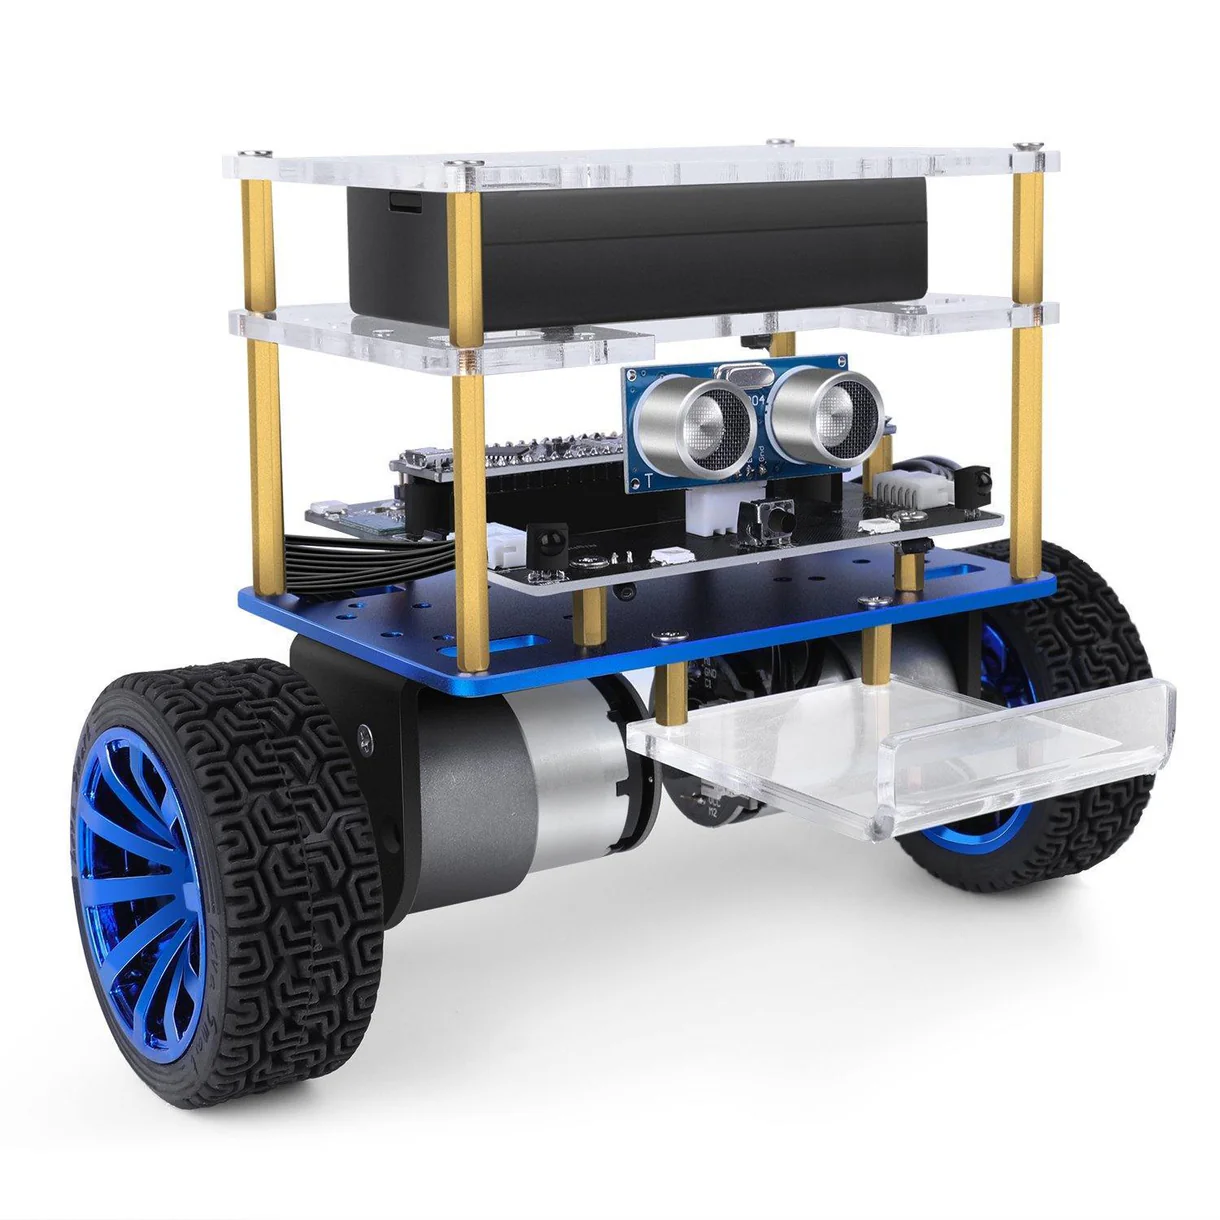
\includegraphics[width=0.7\textwidth, center]{img/elegoo_tumbller.png}
    \caption{Rendering des Elegoo Tumbller}
    \label{fig:elegoo_tumbller}
\end{figure}
\begin{sidewaysfigure}
    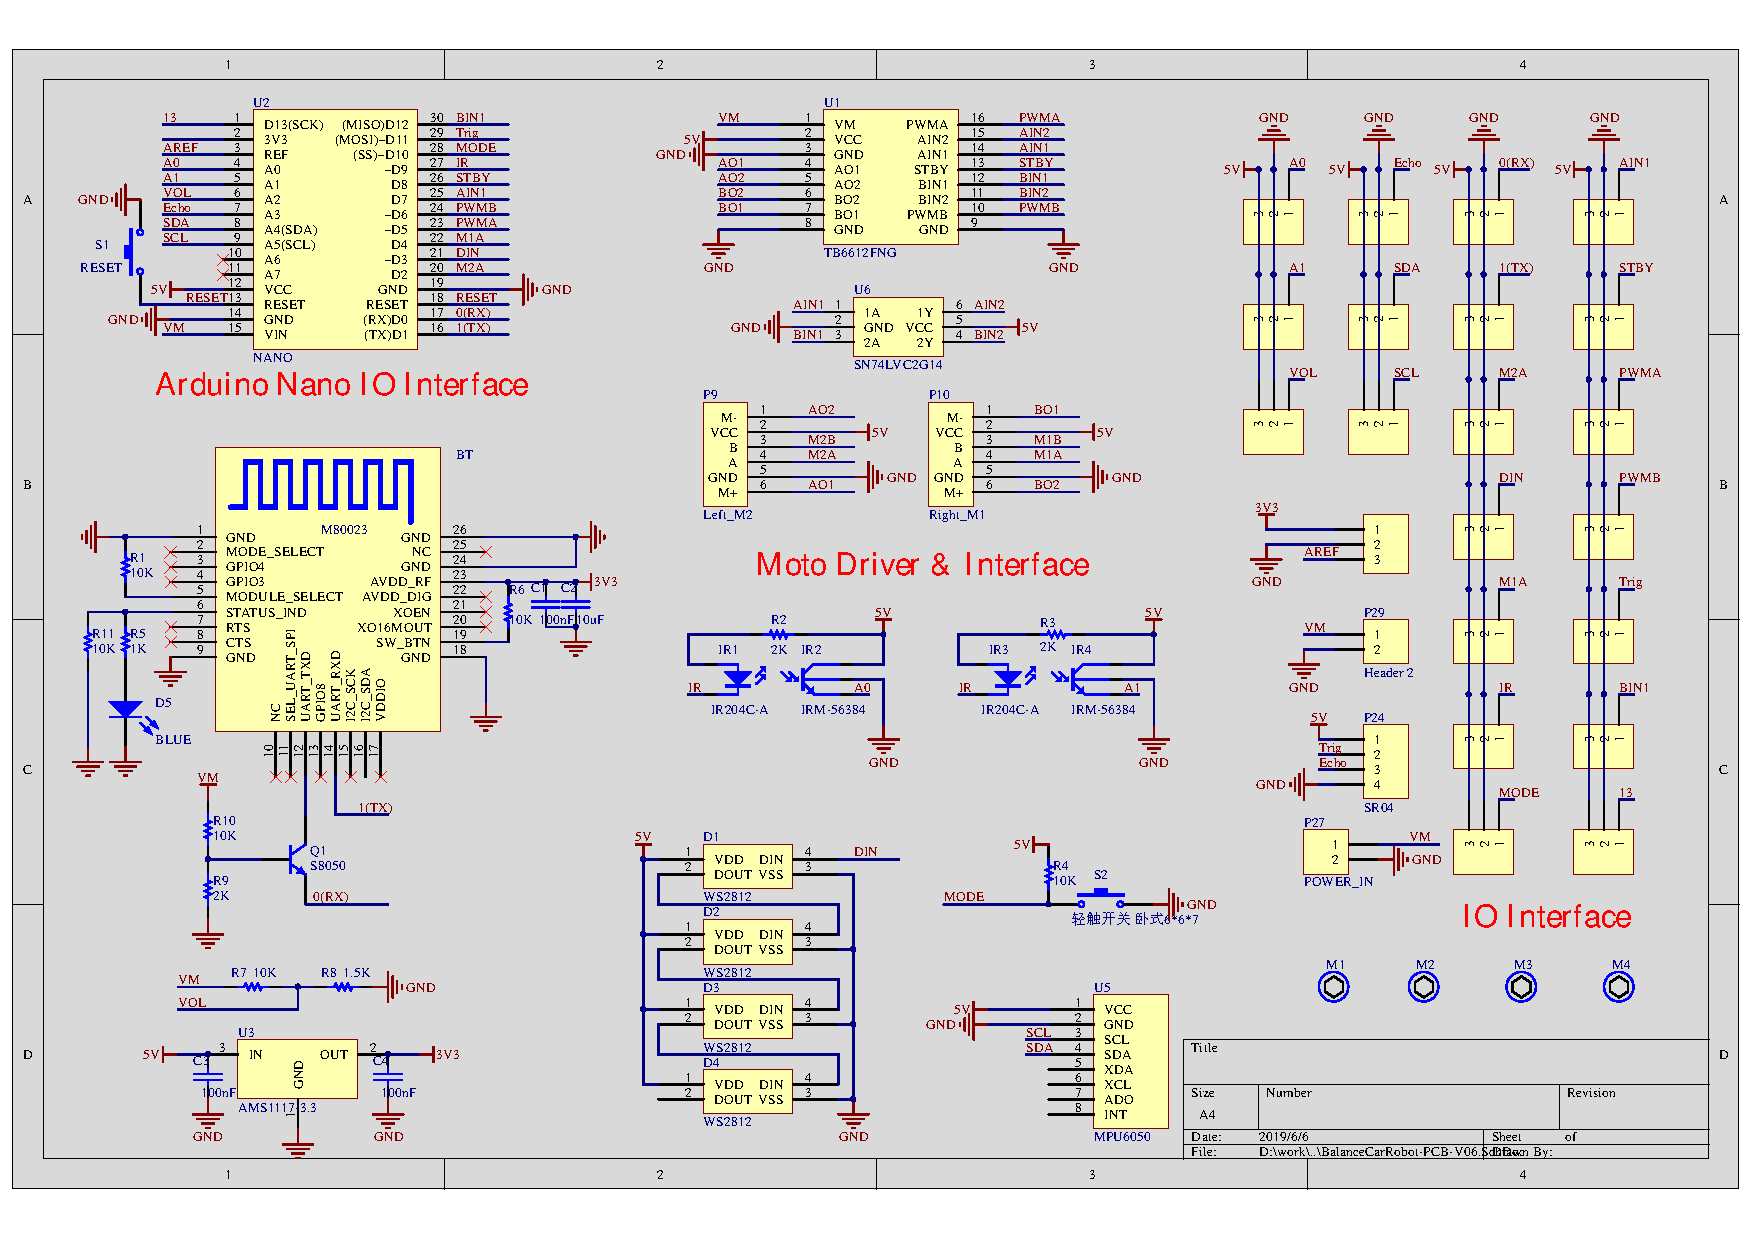
\includegraphics[width=\textwidth, center]{img/elegoo_tumbller_original_circuit.pdf}
    \caption{Originaler Schaltplan des Tumbllers (TODO: neu zeichnen)}
    \label{fig:elegoo_tumbller_original_circuit}
\end{sidewaysfigure}

\section{Guide}
\label{subsec:hardware_guide}
Die Aufgabe von \textit{Guide} ist es,
mithilfe eines LiDAR-Sensors (Siehe Kapitel \ref{subsec:ueberblick_lidar}) die Umgebung nach Hindernissen
und den anderen Robotern abzusuchen.
%
Die vom LiDAR gesammelten Abstandsdaten werden über eine TCP/IP Websocket-Verbindung
an einen zentralen Server weitergegeben,
welcher diese weiter verarbeitet.
%
Um den LiDAR-Sensor zu montieren,
haben wir das Fahrgestell leicht modifiziert
und die oberste Ebene (mit dem Akku) erhöht,
um Platz für Schrauben zu schaffen.

\section{Tamerlan \& Bambi}
\label{subsec:hardware_tamerlan_bambi}